\documentclass[conference]{IEEEtran}
\IEEEoverridecommandlockouts
\usepackage{cite}
\usepackage{balance}
\usepackage{amsmath,amssymb,amsfonts}
\usepackage{graphicx}
\usepackage{textcomp}
\usepackage{xcolor}
\usepackage{booktabs}
\usepackage{algorithm}
\usepackage{algorithmic}
\usepackage{tikz}
\usetikzlibrary{positioning,arrows.meta,fit,calc}
\usepackage[hidelinks]{hyperref}
\newcommand{\NInst}{30}
\newcommand{\NFeasInst}{30}
\newcommand{\NBinding}{12}
\newcommand{\MeanFeasAssign}{45.0}
\newcommand{\Shots}{32}
\newcommand{\UniBits}{0.00033}
\newcommand{\UniOneHot}{0.0169}
\newcommand{\ExactMs}{0.90}
\newcommand{\SAOpt}{10.0}
\newcommand{\SAFeas}{83.3}
\newcommand{\SAMs}{2.3}
\newcommand{\GreedyOpt}{93.3}
\newcommand{\GreedyFeas}{100.0}
\newcommand{\QuboExact}{93.3}
\newcommand{\QXMeanOnePopt}{0.004}
\newcommand{\QXMeanOnePfeas}{0.074}
\newcommand{\QXMeanOneSucc}{12.2}
\newcommand{\QXMeanOneArgmax}{36.7}
\newcommand{\QXMeanOneNfev}{96}
\newcommand{\QXMeanOneMs}{0.29}
\newcommand{\QXMeanTwoPopt}{0.011}
\newcommand{\QXMeanTwoPfeas}{0.249}
\newcommand{\QXMeanTwoSucc}{27.6}
\newcommand{\QXMeanTwoArgmax}{40.0}
\newcommand{\QXMeanTwoNfev}{479}
\newcommand{\QXMeanTwoMs}{4.22}
\newcommand{\QXMeanThreePopt}{0.024}
\newcommand{\QXMeanThreePfeas}{0.439}
\newcommand{\QXMeanThreeSucc}{48.2}
\newcommand{\QXMeanThreeArgmax}{26.7}
\newcommand{\QXMeanThreeNfev}{721}
\newcommand{\QXMeanThreeMs}{4.03}
\newcommand{\QXMeanFourPopt}{0.040}
\newcommand{\QXMeanFourPfeas}{0.547}
\newcommand{\QXMeanFourSucc}{63.7}
\newcommand{\QXMeanFourArgmax}{40.0}
\newcommand{\QXMeanFourNfev}{750}
\newcommand{\QXMeanFourMs}{8.71}
\newcommand{\QXYMeanOnePopt}{0.054}
\newcommand{\QXYMeanOnePfeas}{0.734}
\newcommand{\QXYMeanOneSucc}{67.1}
\newcommand{\QXYMeanOneArgmax}{3.3}
\newcommand{\QXYMeanOneNfev}{272}
\newcommand{\QXYMeanOneMs}{0.83}
\newcommand{\QXYMeanTwoPopt}{0.093}
\newcommand{\QXYMeanTwoPfeas}{0.722}
\newcommand{\QXYMeanTwoSucc}{77.8}
\newcommand{\QXYMeanTwoArgmax}{13.3}
\newcommand{\QXYMeanTwoNfev}{741}
\newcommand{\QXYMeanTwoMs}{2.97}
\newcommand{\QXYMeanThreePopt}{0.143}
\newcommand{\QXYMeanThreePfeas}{0.743}
\newcommand{\QXYMeanThreeSucc}{81.9}
\newcommand{\QXYMeanThreeArgmax}{16.7}
\newcommand{\QXYMeanThreeNfev}{750}
\newcommand{\QXYMeanThreeMs}{3.73}
\newcommand{\QXYMeanFourPopt}{0.215}
\newcommand{\QXYMeanFourPfeas}{0.795}
\newcommand{\QXYMeanFourSucc}{88.4}
\newcommand{\QXYMeanFourArgmax}{40.0}
\newcommand{\QXYMeanFourNfev}{750}
\newcommand{\QXYMeanFourMs}{5.53}
\newcommand{\QXCvarOnePopt}{0.005}
\newcommand{\QXCvarOnePfeas}{0.132}
\newcommand{\QXCvarOneSucc}{14.6}
\newcommand{\QXCvarOneArgmax}{23.3}
\newcommand{\QXCvarOneNfev}{108}
\newcommand{\QXCvarOneMs}{0.37}
\newcommand{\QXCvarTwoPopt}{0.019}
\newcommand{\QXCvarTwoPfeas}{0.294}
\newcommand{\QXCvarTwoSucc}{44.0}
\newcommand{\QXCvarTwoArgmax}{63.3}
\newcommand{\QXCvarTwoNfev}{577}
\newcommand{\QXCvarTwoMs}{54.22}
\newcommand{\QXCvarThreePopt}{0.037}
\newcommand{\QXCvarThreePfeas}{0.356}
\newcommand{\QXCvarThreeSucc}{65.7}
\newcommand{\QXCvarThreeArgmax}{70.0}
\newcommand{\QXCvarThreeNfev}{728}
\newcommand{\QXCvarThreeMs}{793.23}
\newcommand{\QXCvarFourPopt}{0.060}
\newcommand{\QXCvarFourPfeas}{0.376}
\newcommand{\QXCvarFourSucc}{78.4}
\newcommand{\QXCvarFourArgmax}{66.7}
\newcommand{\QXCvarFourNfev}{706}
\newcommand{\QXCvarFourMs}{5.47}
\newcommand{\QXYCvarOnePopt}{0.067}
\newcommand{\QXYCvarOnePfeas}{0.720}
\newcommand{\QXYCvarOneSucc}{82.7}
\newcommand{\QXYCvarOneArgmax}{6.7}
\newcommand{\QXYCvarOneNfev}{241}
\newcommand{\QXYCvarOneMs}{0.83}
\newcommand{\QXYCvarTwoPopt}{0.099}
\newcommand{\QXYCvarTwoPfeas}{0.712}
\newcommand{\QXYCvarTwoSucc}{93.9}
\newcommand{\QXYCvarTwoArgmax}{20.0}
\newcommand{\QXYCvarTwoNfev}{413}
\newcommand{\QXYCvarTwoMs}{1.78}
\newcommand{\QXYCvarThreePopt}{0.127}
\newcommand{\QXYCvarThreePfeas}{0.672}
\newcommand{\QXYCvarThreeSucc}{97.3}
\newcommand{\QXYCvarThreeArgmax}{36.7}
\newcommand{\QXYCvarThreeNfev}{343}
\newcommand{\QXYCvarThreeMs}{1.88}
\newcommand{\QXYCvarFourPopt}{0.149}
\newcommand{\QXYCvarFourPfeas}{0.664}
\newcommand{\QXYCvarFourSucc}{98.1}
\newcommand{\QXYCvarFourArgmax}{50.0}
\newcommand{\QXYCvarFourNfev}{284}
\newcommand{\QXYCvarFourMs}{1.75}
\newcommand{\XYPfeasMin}{0.722}
\newcommand{\XYPfeasMax}{0.795}
\newcommand{\GainXYoverUni}{12.7}
\newcommand{\GainXYoverX}{5.3}
\newcommand{\ZZX}{14.0}
\newcommand{\ZZXY}{2.0}
\newcommand{\OvPairs}{2.0}
\newcommand{\ScaleMaxQ}{18}
\newcommand{\ScaleXYsix}{0.006}
\newcommand{\ScaleUnisix}{0.0017}
\newcommand{\ScaleXYmsSix}{99.4}
\newcommand{\ScaleExactSix}{8.14}
\newcommand{\ScaleQuboMin}{90}
\newcommand{\NNonBinding}{18}
\newcommand{\XYBind}{0.111}
\newcommand{\XYNonBind}{0.284}
\newcommand{\XYMin}{0.002}
\newcommand{\XYCvarMin}{0.074}
\newcommand{\XYMax}{0.796}
\newcommand{\XYCvarMax}{0.439}
\newcommand{\XBind}{0.039}
\newcommand{\XNonBind}{0.041}
\newcommand{\ScaleXYtwo}{0.694}
\newcommand{\ScaleXtwo}{0.124}
\newcommand{\ScaleXsix}{0.0009}
\newcommand{\ScaleInfeasSix}{1}
\newcommand{\ScaleXYfeasSix}{0.271}
\newcommand{\ScaleXfeasSix}{0.051}
\newcommand{\TrajInst}{10}
\newcommand{\TrajRuns}{200}
\newcommand{\TrajIdealXY}{0.172}
\newcommand{\TrajIdealX}{0.046}
\newcommand{\TrajXYOne}{0.105}
\newcommand{\TrajXOne}{0.033}
\newcommand{\TrajGlobXYOne}{0.086}
\newcommand{\TrajXYTwo}{0.058}
\newcommand{\TrajRatioOne}{3.2}
\newcommand{\NtwoLayer}{14.0}
\newcommand{\CnotLayer}{28}
\newcommand{\CnotFour}{112}
\newcommand{\ExOpt}{ABCB}
\newcommand{\ExOptCost}{80.86}
\newcommand{\ExSecond}{ABBB}
\newcommand{\ExSecondCost}{80.88}
\newcommand{\ExGap}{0.02}
\newcommand{\ExXYOpt}{0.319}
\newcommand{\ExXYSecond}{0.303}
\newcommand{\ExXYFeas}{0.982}
\newcommand{\ExXOpt}{0.049}
\newcommand{\ExXFeas}{0.681}
\newcommand{\ExNFeas}{29}
\newcommand{\NoiseXYOnePct}{0.104}
\newcommand{\NoiseXYOnePctDepth}{4}
\newcommand{\NoiseXOnePct}{0.023}
\newcommand{\NoiseXYTwoPct}{0.050}
\newcommand{\NoiseXYTwoPctDepth}{4}
\newcommand{\NoiseCvarTwoPctDepth}{2}

\newtheorem{lemma}{Lemma}

\begin{document}

\title{Constraint-Preserving QAOA for Flood Shelter\\
Assignment: A Statevector Study on\\
Digital-Twin Instances}

%<AUTHORS>
\author{
\IEEEauthorblockN{Nandhakumar T}
\IEEEauthorblockA{\textit{Department of Information Technology}\\
\textit{Sona College of Technology}\\
Salem, Tamil Nadu, India\\
nandhakumartm93@gmail.com}
\and
\IEEEauthorblockN{Balakarthikeyan B S}
\IEEEauthorblockA{\textit{Department of Artificial Intelligence and Data Science}\\
\textit{Sona College of Technology}\\
Salem, Tamil Nadu, India\\
balasan2626@gmail.com}
\and
\IEEEauthorblockN{Gowthaman J}
\IEEEauthorblockA{\textit{Department of Artificial Intelligence and Data Science}\\
\textit{Sona College of Technology}\\
Salem, Tamil Nadu, India\\
gowthamanjanadhran@gmail.com}
\and
\IEEEauthorblockN{Abhishek S}
\IEEEauthorblockA{\textit{Department of Artificial Intelligence and Data Science}\\
\textit{Sona College of Technology}\\
Salem, Tamil Nadu, India\\
abisheksengodan18@gmail.com}
}
%</AUTHORS>

\maketitle

\begin{abstract}
Assigning evacuation groups to shelters under road closures and limited capacity is a small constrained combinatorial problem, and it is often cited as a target for quantum optimization. We test this claim on instances taken from a flood digital twin rather than on random graphs. Each instance assigns four groups to three shelters after a road closure and a shelter surge, giving a 12-qubit quadratic unconstrained binary optimization (QUBO) problem. We compare the Quantum Approximate Optimization Algorithm (QAOA) with the standard transverse-field mixer against a constraint-preserving ring-XY mixer, each trained on the mean energy and on the conditional value-at-risk (CVaR), at depths 1 to 4, using exact noiseless statevector simulation. On \NFeasInst{} feasible instances, the XY mixer placed \QXYMeanFourPopt{} of its probability on the optimal plan at depth 4, compared with \QXMeanFourPopt{} for the standard mixer and \UniOneHot{} for uniform sampling of one-hot plans, and it kept most of its probability on feasible plans at every depth. CVaR training raised the chance of finding the optimum within a fixed number of shots for both mixers. In a gate-level simulation with a 1\% two-qubit Pauli error rate, the XY mixer still reached $P_{\mathrm{opt}}=\TrajXYOne$, against \TrajXOne{} for the standard mixer. Classical methods remain far ahead at this size: exhaustive search solved every instance in \ExactMs~ms. A scaling run up to \ScaleMaxQ{} qubits shows how quickly simulation cost grows. We claim no quantum advantage. The study shows which design choices matter if such problems are moved to quantum hardware.
\end{abstract}

\begin{IEEEkeywords}
QAOA, quantum alternating operator ansatz, XY mixer, QUBO, CVaR, evacuation planning, shelter assignment, digital twin
\end{IEEEkeywords}

\section{Introduction}
When a flood closes roads and fills shelters, an emergency officer must decide again which shelter each evacuation group should go to. The decision couples travel time, flood exposure along the route and the seats left at each shelter. Written as a binary program, it becomes a constrained assignment problem of the kind that is routinely encoded as a QUBO or Ising model \cite{Lucas2014,Glover2019} and offered as an application for near-term quantum optimization \cite{Cadelina2024,Abbas2024}.

Two questions are usually left open in such proposals. The first is whether the quantum circuit respects the constraints or merely penalises their violation. In the original QAOA \cite{Farhi2014}, constraints enter the cost function as penalties and the transverse-field mixer explores all $2^n$ bitstrings, most of which are not valid plans. The quantum alternating operator ansatz \cite{Hadfield2019} instead uses mixers that keep the state inside the feasible subspace of one-hot constraints, such as XY mixers \cite{WangZ2020,Fuchs2022}. The second question is how the result compares with ordinary classical methods on instances of realistic shape. Benchmarks on random graphs do not answer it for evacuation.

We address both questions on instances generated by the digital twin of a flood decision-support prototype. Our contributions are:
\begin{enumerate}
\item A QUBO formulation of shelter assignment built from twin state, with a pairwise capacity encoding, a penalty bound that makes every violation more expensive than any feasible plan, and a measured exactness rate for the encoding.
\item A controlled comparison of the transverse-field and ring-XY mixers, under mean-energy and CVaR training \cite{Barkoutsos2020}, at depths 1--4 on \NFeasInst{} instances, using exact statevector simulation.
\item A scaling study from 6 to \ScaleMaxQ{} qubits and a comparison with exhaustive search, simulated annealing \cite{Kirkpatrick1983} and a greedy rule.
\end{enumerate}
All results are from classical simulation of noiseless circuits. We make no claim of quantum speed-up, and the classical baselines are reported because they are faster.

\section{Related Work}
\textit{Formulations.} Lucas gave Ising forms for many NP-hard problems \cite{Lucas2014}, and Glover \textit{et al.} describe how assignment and capacity constraints become quadratic penalties \cite{Glover2019}. Shelter location and allocation for flood evacuation has long been studied with classical integer programming \cite{Sherali1991}. Quantum annealing has been applied to disaster resource allocation \cite{Cadelina2024}.

\textit{QAOA and mixers.} QAOA alternates a cost unitary and a mixing unitary for $p$ layers \cite{Farhi2014}. Hadfield \textit{et al.} generalised the mixer so that it preserves hard constraints \cite{Hadfield2019}. Wang \textit{et al.} analysed ring and complete XY mixers for one-hot constraints \cite{WangZ2020}, and Fuchs \textit{et al.} gave a general construction of constraint-preserving mixers \cite{Fuchs2022}. Preparing the initial superposition of one-hot states requires W-state circuits \cite{Bartschi2019}.

\textit{Training and limits.} Zhou \textit{et al.} proposed interpolating optimal angles from depth $p$ to $p{+}1$ (INTERP) \cite{Zhou2020}, and Barkoutsos \textit{et al.} showed that optimising the CVaR of the energy, rather than its mean, increases the probability of good samples \cite{Barkoutsos2020}. Warm starts from classical solutions are another option \cite{Egger2021}. Most published comparisons of mixers and objectives use MaxCut or random constrained instances. Shelter assignment differs in two ways that matter for QAOA: its costs come from travel times that are close to each other, so the optimum is separated from many near-optimal plans by small energy gaps, and its capacity constraints couple groups that would otherwise be independent. We therefore evaluate on instances produced by the same digital twin that drives the decision-support prototype, after the same disruption the twin uses in its routing benchmark. On current processors, QAOA performance falls with problem size and circuit depth \cite{Harrigan2021}, and reviews of noisy intermediate-scale quantum (NISQ) algorithms stress that practical advantage in optimization has not been shown \cite{Preskill2018,Bharti2022,Abbas2024}.

\textit{Research gap.} The mixer and objective studies above use MaxCut-style or random instances, and the disaster-response work \cite{Cadelina2024} solves a penalty QUBO on an annealer without comparing formulations. To our knowledge, constraint-preserving QAOA has not been evaluated on capacity-constrained evacuation instances against an exact optimum, classical baselines and a gate-level noise model together. This paper provides that evaluation.

\section{Problem Formulation}
\subsection{Instances from the Digital Twin}
The twin models a corridor with three population zones, nine junctions and three shelters joined by 22 roads. Every road carries a travel time, a flood-depth index and a congestion level drawn from a fixed seed. Shelters have capacities of 120, 90 and 70 people with an initial occupancy of 15--45\%, and groups have 8--22 people. Each instance applies the disruption used in the twin's routing benchmark: road R5 closes and Shelter A receives arrivals equal to half its capacity. For group $g$ and shelter $s$ we take the best open path under the twin's flood- and congestion-weighted edge cost, and define
\begin{equation}
c_{gs}=T_{gs}+5H_{gs},
\end{equation}
where $T_{gs}$ is travel time in minutes and $H_{gs}$ is the mean flood index along the path. The pair $(g,s)$ is \emph{forbidden} if no open path exists, the shelter has failed, or the group alone exceeds the remaining seats $R_s$. With $G$ groups, binary variables $x_{gs}$ give $n=3G$ qubits. A plan is feasible if every group has exactly one shelter, no forbidden pair is used and $\sum_g n_g x_{gs}\le R_s$ for each shelter, where $n_g$ is the group size.

\subsection{QUBO with Pairwise Capacity}
The capacity constraint is linear in $x$ but has an inequality, which normally needs slack qubits \cite{Glover2019}. We use a pairwise encoding instead. Let $\mathcal{O}=\{(g,h,s): n_g+n_h>R_s\}$ be the pairs of groups that cannot share shelter $s$. With shifted costs $c'_{gs}=c_{gs}-\min_{s'}c_{gs'}$, the energy is
\begin{multline}
E(\mathbf{x})=\sum_{g,s}c'_{gs}x_{gs}+P\Big[\sum_g\Big(1-\sum_s x_{gs}\Big)^2\\
+\sum_{(g,s)\in\mathcal{F}}x_{gs}+\sum_{(g,h,s)\in\mathcal{O}}x_{gs}x_{hs}\Big],
\label{eq:qubo}
\end{multline}
where $\mathcal{F}$ is the set of forbidden pairs.

\begin{lemma}
With $P=1+\sum_g\max_s c'_{gs}$, every bitstring that breaks a one-hot, forbidden-pair or pairwise-capacity term has higher energy than every bitstring that breaks none of them.
\end{lemma}
\noindent\textit{Proof.} Since $c'_{gs}\ge0$, a bitstring with no violated term has energy at most $P-1$. A violated term adds at least $P$, and the cost part is non-negative. \hfill$\blacksquare$

\smallskip
On one-hot states, the shift subtracts the constant $\sum_g\min_s c_{gs}$, so the optimal plan is unchanged, but the energy scale now reflects only the decision being made. Without the shift, the penalty dominated the energy and QAOA learned feasibility but not cost in our preliminary runs. The pairwise encoding is exact when no three groups overload a shelter that each pair could share. When that fails, the QUBO minimiser can be infeasible, so every plan is re-checked exactly before use. We report how often the minimiser of (\ref{eq:qubo}) is the true optimum.

\section{QAOA Variants}
For depth $p$ and angles $(\boldsymbol\gamma,\boldsymbol\beta)$, QAOA prepares
\begin{equation}
|\psi(\boldsymbol\gamma,\boldsymbol\beta)\rangle=\prod_{k=1}^{p}e^{-i\beta_k B}\,e^{-i\gamma_k \hat E/\Delta}\,|\psi_0\rangle,
\end{equation}
where $\hat E$ is diagonal with entries $E(\mathbf{x})$ and $\Delta=P-1$ normalises feasible energies to $[0,1]$. Substituting $x_q=(1-Z_q)/2$ turns (\ref{eq:qubo}) into an Ising Hamiltonian
\begin{equation}
\hat E=\sum_{q}h_qZ_q+\sum_{q<r}J_{qr}Z_qZ_r+\mathrm{const},
\label{eq:ising}
\end{equation}
so the cost unitary needs one single-qubit $R_Z$ rotation per qubit and one two-qubit $ZZ$ rotation per non-zero $J_{qr}$. Each quadratic term of (\ref{eq:qubo}), whether from the one-hot penalty or from an overloaded pair, therefore adds a two-qubit gate to every layer.

\textit{Transverse-field (X) mixer.} $B=\sum_q X_q$ and $|\psi_0\rangle=|+\rangle^{\otimes n}$. All $2^{n}$ bitstrings are reachable, and constraints act only through the penalties in (\ref{eq:qubo}).

\textit{Ring-XY mixer.} For each group $g$ with qubits $a_g,b_g,c_g$,
\begin{equation}
B_{\mathrm{XY}}=\sum_{g}\ \sum_{(u,v)\in\{(a_g,b_g),(b_g,c_g),(c_g,a_g)\}}\tfrac12\big(X_uX_v+Y_uY_v\big).
\label{eq:xy}
\end{equation} Each term swaps amplitude between $|01\rangle$ and $|10\rangle$ and conserves the number of ones, so a one-hot group stays one-hot \cite{WangZ2020}. The start state is a product of W states, $|W_3\rangle^{\otimes G}$ with $|W_3\rangle=(|100\rangle+|010\rangle+|001\rangle)/\sqrt3$, which is the uniform superposition of the $3^G$ one-hot plans. The one-hot penalty is then constant and is dropped, which also removes $3G$ two-qubit cost terms per layer. The three ring terms do not commute and are applied in a fixed order, as in a first-order Trotter step.

\textit{Training.} We minimise either the mean energy $\langle\hat E\rangle$ or the conditional value-at-risk with $\alpha=0.1$ \cite{Barkoutsos2020}. Sorting bitstrings by energy, $E_{(1)}\le E_{(2)}\le\dots$, with measurement probabilities $\pi_{(k)}$ and cumulative mass $\Pi_k=\sum_{j\le k}\pi_{(j)}$,
\begin{equation}
\mathrm{CVaR}_\alpha=\frac1\alpha\sum_k E_{(k)}\,\min\!\big(\pi_{(k)},\ \max(0,\ \alpha-\Pi_{k-1})\big),
\label{eq:cvar}
\end{equation}
the mean energy of the lowest $\alpha$ probability mass. Minimising it rewards the circuit for placing some probability on low-energy plans even when the rest of the distribution is poor. Angles are optimised by COBYLA \cite{Powell1994} with at most 250 evaluations per start. At $p=1$ we use two random starts. At $p>1$ we add an INTERP start built from the $p-1$ optimum \cite{Zhou2020} to two random starts and keep the best (Algorithm~\ref{alg:train}). Fig.~\ref{fig:flow} summarises the pipeline.

\begin{algorithm}[t]
\caption{Depth-progressive QAOA training}
\label{alg:train}
\begin{algorithmic}[1]
\small
\STATE build $\hat E/\Delta$ from (\ref{eq:qubo}); choose mixer $B$ and $|\psi_0\rangle$
\STATE $\boldsymbol\theta^{(0)}\leftarrow\emptyset$
\FOR{$p=1$ \TO $4$}
\STATE starts $\leftarrow$ two draws $\gamma_k\sim U(0,\pi)$, $\beta_k\sim U(0,\pi/2)$
\IF{$p>1$}
\STATE add INTERP$(\boldsymbol\theta^{(p-1)})$ to starts
\ENDIF
\STATE $\boldsymbol\theta^{(p)}\leftarrow$ best COBYLA result over starts on $\langle\hat E\rangle$ or (\ref{eq:cvar})
\STATE record $P_{\mathrm{opt}}$, $P_{\mathrm{feas}}$ and evaluations for $\boldsymbol\theta^{(p)}$
\ENDFOR
\end{algorithmic}
\end{algorithm}

\begin{figure}[t]
\centering
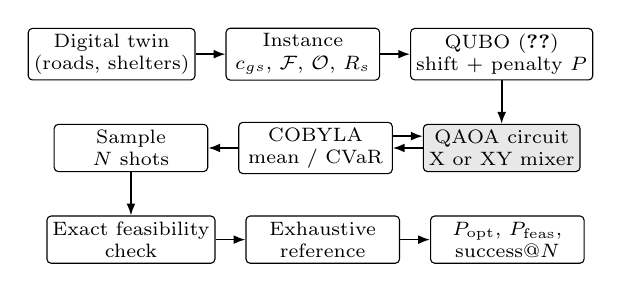
\begin{tikzpicture}[
  font=\scriptsize,
  box/.style={draw, rounded corners=1.5pt, align=center, minimum width=1.95cm, minimum height=0.6cm, inner sep=2pt},
  q/.style={box, fill=gray!18},
  arr/.style={-{Latex[length=1.5mm]}, semithick}]
\node[box] (tw) {Digital twin\\(roads, shelters)};
\node[box, right=0.38cm of tw] (ins) {Instance\\$c_{gs}$, $\mathcal{F}$, $\mathcal{O}$, $R_s$};
\node[box, right=0.38cm of ins] (qb) {QUBO (\ref{eq:qubo})\\shift + penalty $P$};
\node[q, below=0.55cm of qb] (circ) {QAOA circuit\\X or XY mixer};
\node[box, left=0.38cm of circ] (opt) {COBYLA\\mean / CVaR};
\node[box, left=0.38cm of opt] (samp) {Sample\\$N$ shots};
\node[box, below=0.55cm of samp] (ver) {Exact feasibility\\check};
\node[box, right=0.38cm of ver] (ref) {Exhaustive\\reference};
\node[box, right=0.38cm of ref] (met) {$P_{\mathrm{opt}}$, $P_{\mathrm{feas}}$,\\success@$N$};
\draw[arr] (tw) -- (ins);
\draw[arr] (ins) -- (qb);
\draw[arr] (qb) -- (circ);
\draw[arr] (circ.west) -- (opt.east);
\draw[arr] ([yshift=1.5mm]opt.east) -- ([yshift=1.5mm]circ.west);
\draw[arr] (opt) -- (samp);
\draw[arr] (samp) -- (ver);
\draw[arr] (ver) -- (ref);
\draw[arr] (ref) -- (met);
\end{tikzpicture}
\caption{Experimental pipeline. The shaded block is simulated exactly as a statevector. Every sampled plan is checked against the exact constraints, and the exhaustive reference gives the optimum.}
\label{fig:flow}
\end{figure}

\subsection{Simulator}
The simulator stores the $2^{n}$ complex amplitudes in double precision and applies each layer directly. The cost unitary is diagonal, so it is one elementwise multiplication by $e^{-i\gamma_k E(\mathbf{x})/\Delta}$ with the energies of all bitstrings computed once per instance. The transverse-field mixer applies $R_X(2\beta_k)$ to one qubit at a time by reshaping the amplitude vector so that the target qubit becomes a length-2 axis. Each XY term mixes only the amplitude pairs whose two target bits are $01$ and $10$; we precompute those index pairs once and update them with a $2\times2$ rotation. One objective evaluation at 12 qubits takes under ten milliseconds on a laptop, so the cost of training is dominated by the number of objective evaluations, which we report. All random choices (instances, restarts, sampling and noise) use fixed seeds.

\section{Experimental Setup}
We generated \NInst{} instances from the twin with seeds $42+17i$, $i=0,\dots,29$, and used the first four groups ($G=4$, $n=12$). All \NFeasInst{} instances had at least one feasible plan, on average \MeanFeasAssign{} of the 81 one-hot plans. In \NBinding{} instances, sending every group to its cheapest shelter overloaded a shelter, so capacity changed the optimal plan. All circuits were simulated as exact $2^{n}$-amplitude statevectors in double precision, without noise or shot noise during training.

We report three metrics: $P_{\mathrm{opt}}$, the probability of measuring an optimal plan; $P_{\mathrm{feas}}$, the probability of measuring a feasible plan; and success@$N$, the probability that at least one of $N=\Shots$ shots is optimal, $1-(1-P_{\mathrm{opt}})^{N}$. We also count objective evaluations, since each one corresponds to a batch of circuit executions on hardware. The baselines are uniform sampling of all $2^{12}$ bitstrings ($P_{\mathrm{opt}}=\UniBits$ on average) and of the 81 one-hot plans ($\UniOneHot$); exhaustive search; single-bit-flip simulated annealing on (\ref{eq:qubo}) with one restart of 60 sweeps; and a greedy rule that places the largest group first in its cheapest shelter with seats left. The scaling study used the first ten instances with $G=2,\dots,6$ ($n=6,\dots,18$), the mean objective and $p=2$.

\section{Results}
\subsection{Mixer and Objective}
Table~\ref{tab:main} and Fig.~\ref{fig:popt} give the main results. The XY mixer was better on both metrics. At $p=4$ with the mean objective it reached $P_{\mathrm{opt}}=\QXYMeanFourPopt$, which is \GainXYoverUni{} times uniform one-hot sampling and \GainXYoverX{} times the X mixer at the same depth. Because its state never leaves the one-hot subspace, its feasibility probability depended only on capacity and forbidden pairs, and it stayed between \XYPfeasMin{} and \XYPfeasMax{} across depths. The X mixer started with almost all of its probability on invalid bitstrings ($P_{\mathrm{feas}}=\QXMeanOnePfeas$ at $p=1$) and needed every added layer to recover feasibility. With \Shots{} shots, the XY mixer at $p=4$ found the optimal plan with probability \QXYMeanFourSucc\%, against \QXMeanFourSucc\% for the X mixer.

CVaR training raised the X mixer's $P_{\mathrm{opt}}$ to \QXCvarFourPopt{} at $p=4$, because it rewards the low-energy tail even when most of the state is infeasible. For the XY mixer, CVaR lowered the mean $P_{\mathrm{opt}}$ at $p=4$ to \QXYCvarFourPopt{} but raised success@\Shots{} from \QXYMeanFourSucc\% to \QXYCvarFourSucc\%. Because success@$N$ grows sublinearly with $P_{\mathrm{opt}}$, a higher mean success with a lower mean $P_{\mathrm{opt}}$ means that CVaR left fewer instances with a very small $P_{\mathrm{opt}}$. If the plan is chosen as the best of a batch of shots, as it would be in practice, CVaR is the better objective for both mixers. Deeper circuits needed more evaluations: \QXYMeanFourNfev{} on average for the XY mixer at $p=4$, including the restarts at lower depths.

\begin{table}[t]
\caption{QAOA on \NFeasInst{} twin instances (12 qubits), mean over instances}
\label{tab:main}
\centering
\footnotesize
\setlength{\tabcolsep}{3.2pt}
\begin{tabular}{llccccc}
\toprule
Mixer & Objective & $p$ & $P_{\mathrm{opt}}$ & $P_{\mathrm{feas}}$ & succ@\Shots{} (\%) & Evals\\
\midrule
X & mean & 1 & 0.004 & 0.074 & 12.2 & 96\\
X & mean & 2 & 0.011 & 0.249 & 27.6 & 479\\
X & mean & 3 & 0.024 & 0.439 & 48.2 & 721\\
X & mean & 4 & 0.040 & 0.547 & 63.7 & 750\\
\addlinespace[1pt]
XY & mean & 1 & 0.054 & 0.734 & 67.1 & 272\\
XY & mean & 2 & 0.093 & 0.722 & 77.8 & 741\\
XY & mean & 3 & 0.143 & 0.743 & 81.9 & 750\\
XY & mean & 4 & 0.215 & 0.795 & 88.4 & 750\\
\addlinespace[1pt]
X & CVaR$_{0.1}$ & 1 & 0.005 & 0.132 & 14.6 & 108\\
X & CVaR$_{0.1}$ & 2 & 0.019 & 0.294 & 44.0 & 577\\
X & CVaR$_{0.1}$ & 3 & 0.037 & 0.356 & 65.7 & 728\\
X & CVaR$_{0.1}$ & 4 & 0.060 & 0.376 & 78.4 & 706\\
\addlinespace[1pt]
XY & CVaR$_{0.1}$ & 1 & 0.067 & 0.720 & 82.7 & 241\\
XY & CVaR$_{0.1}$ & 2 & 0.099 & 0.712 & 93.9 & 413\\
XY & CVaR$_{0.1}$ & 3 & 0.127 & 0.672 & 97.3 & 343\\
XY & CVaR$_{0.1}$ & 4 & 0.149 & 0.664 & 98.1 & 284\\
\bottomrule
\multicolumn{7}{l}{\scriptsize Uniform one-hot sampling: $P_{\mathrm{opt}}=\UniOneHot$. Evals = objective evaluations at depth $p$.}\\
\end{tabular}
\end{table}

\begin{figure}[t]
\centering
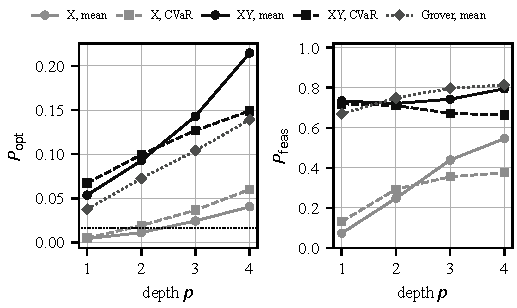
\includegraphics[width=\columnwidth]{fig_popt.pdf}
\caption{Probability of the optimal plan (left) and of any feasible plan (right) against depth. The dotted line is uniform sampling of one-hot plans.}
\label{fig:popt}
\end{figure}

\subsection{Instance Difficulty}
The means in Table~\ref{tab:main} hide a wide spread between instances (Table~\ref{tab:bind}). With the mean objective at $p=4$, the XY mixer's $P_{\mathrm{opt}}$ ranged from \XYMin{} to \XYMax. It was \XYNonBind{} on the \NNonBinding{} instances where every group could use its cheapest shelter, and fell to \XYBind{} on the \NBinding{} instances where capacity forced at least one group elsewhere. In these instances the optimum is a less obvious plan and has to be separated from cheaper plans that overload a shelter. The X mixer was uniformly poor (\XNonBind{} and \XBind), so capacity did not change its result much. CVaR changed the shape of the XY distribution more than its mean: it raised the worst instance from \XYMin{} to \XYCvarMin{} and lowered the best from \XYMax{} to \XYCvarMax. This explains why CVaR improved success within \Shots{} shots while lowering the mean $P_{\mathrm{opt}}$. Fig.~\ref{fig:inst} shows the individual instances: the XY results with the mean objective include a few instances with $P_{\mathrm{opt}}$ near zero, all of them capacity-bound, and CVaR removes that tail.

\begin{figure}[t]
\centering
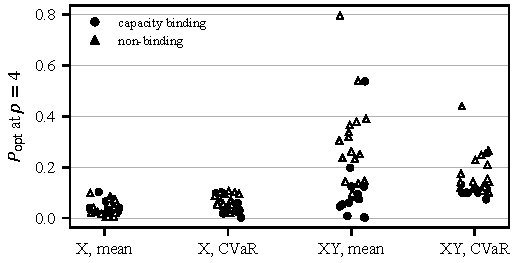
\includegraphics[width=\columnwidth]{fig_inst.pdf}
\caption{$P_{\mathrm{opt}}$ at depth 4 for each of the \NFeasInst{} instances. Filled circles: capacity changes the optimal plan; open triangles: it does not.}
\label{fig:inst}
\end{figure}

\begin{table}[t]
\caption{$P_{\mathrm{opt}}$ at $p=4$ by instance type and its spread over instances}
\label{tab:bind}
\centering
\footnotesize
\setlength{\tabcolsep}{3pt}
\begin{tabular}{lccccc}
\toprule
 & \multicolumn{2}{c}{Mean} & \multicolumn{3}{c}{Over all instances}\\
Variant & non-binding & binding & min & median & max\\
\midrule
X, mean & 0.041 & 0.039 & 0.005 & 0.035 & 0.102\\
X, CVaR & 0.074 & 0.039 & 0.002 & 0.057 & 0.106\\
XY, mean & 0.284 & 0.111 & 0.002 & 0.145 & 0.796\\
XY, CVaR & 0.170 & 0.117 & 0.074 & 0.120 & 0.439\\
\bottomrule
\multicolumn{6}{l}{\scriptsize binding = capacity changes the optimal plan (\NBinding{} instances); non-binding: \NNonBinding.}\\
\end{tabular}
\end{table}

\subsection{A Worked Instance}
Table~\ref{tab:example} shows the first instance (seed 42) after the disruption. Shelter A has only 19 seats left, so groups G3 and G4, with 21 and 20 people, cannot use it at all, and G1 can use it only on its own. Of the 81 one-hot plans, \ExNFeas{} are feasible. The optimal plan, written as the shelter of G1--G4, is \ExOpt{} at \ExOptCost{} minutes, and the greedy rule also finds it. The runner-up, \ExSecond, costs \ExSecondCost{} minutes, only \ExGap{} minutes more.

\begin{table}[t]
\caption{Worked instance (seed 42): route cost $c_{gs}$ (min) after the disruption; -- marks a forbidden pair}
\label{tab:example}
\centering
\footnotesize
\setlength{\tabcolsep}{5pt}
\begin{tabular}{lcccc}
\toprule
Group & $n_g$ & Shelter A & Shelter B & Shelter C\\
\midrule
G1 & 18 & 16.62 & 23.58 & 28.89\\
G2 & 13 & 21.54 & 20.37 & 24.97\\
G3 & 21 & -- & 20.31 & 20.30\\
G4 & 20 & -- & 23.58 & 28.89\\
\midrule
Seats left & & 19 & 76 & 54\\
\bottomrule
\end{tabular}
\end{table}

Table~\ref{tab:top} lists the most likely measurements of the trained depth-4 circuits. The XY circuit placed \ExXYOpt{} of its probability on the optimum and \ExXYSecond{} on the runner-up, and almost all of the rest on other feasible plans (total \ExXYFeas). The X circuit put only \ExXOpt{} on the optimum and \ExXFeas{} on feasible plans. The near-tie between the two best plans is typical of these instances: travel times of alternative routes are close, so the energy gap that QAOA must resolve is small, and a sampler that finds the runner-up has still found a good plan. This is also why success within a batch of shots is a more useful measure than $P_{\mathrm{opt}}$ alone.

\begin{table}[t]
\caption{Five most likely plans of the trained XY circuit for the worked instance, and their probability under the X circuit}
\label{tab:top}
\centering
\footnotesize
\setlength{\tabcolsep}{5pt}
\begin{tabular}{lcccl}
\toprule
Plan (G1--G4) & Cost (min) & XY prob. & X prob. & \\
\midrule
ABCB & 80.86 & 0.319 & 0.049 & optimal\\
ABBB & 80.88 & 0.303 & 0.049 & \\
BBCB & 87.82 & 0.060 & 0.035 & \\
BBBB & 87.83 & 0.057 & 0.035 & \\
ACCB & 85.47 & 0.046 & $<$0.035 & \\
\bottomrule
\end{tabular}
\end{table}

\subsection{Encoding and Circuit Resources}
The minimiser of (\ref{eq:qubo}) was the true optimum in \QuboExact\% of the main instances. On average an instance had \OvPairs{} overloaded pairs. Per layer, the X-mixer cost unitary needed \ZZX{} two-qubit $ZZ$ rotations, while the XY variant needed \ZZXY{}, because the one-hot penalty disappears. The XY mixer itself adds three two-qubit XY rotations per group and layer, and the W-state preparation adds a fixed overhead at the start \cite{Bartschi2019}. Table~\ref{tab:res} summarises the per-layer gate budget for the 12-qubit instances. The two variants need exactly the same number of two-qubit gates per layer: the 12 one-hot couplings of the X variant become 12 XY rotations. The XY mixer's advantage in Table~\ref{tab:main} therefore does not come from a larger circuit. Compiled to CNOT gates, each $ZZ$ rotation and each XY rotation needs two CNOTs, so one layer needs about \CnotLayer{} CNOTs and a depth-4 circuit about \CnotFour{}, plus the W-state preparation for the XY variant. These counts assume all-to-all connectivity; routing on a device with nearest-neighbour coupling would add SWAP gates.

\begin{table}[t]
\caption{Gates per QAOA layer, 12-qubit instances (mean over instances)}
\label{tab:res}
\centering
\footnotesize
\setlength{\tabcolsep}{4pt}
\begin{tabular}{lcc}
\toprule
Gate & X mixer & XY mixer\\
\midrule
Cost: single-qubit $R_Z$ & 12 & 12\\
Cost: two-qubit $ZZ$ & \ZZX & \ZZXY\\
Mixer: single-qubit $R_X$ & 12 & 0\\
Mixer: two-qubit XY & 0 & 12\\
Initial state & $H^{\otimes 12}$ & $|W_3\rangle^{\otimes 4}$\\
\bottomrule
\end{tabular}
\end{table}

\subsection{Sensitivity to Gate Noise}\label{sec:noise}
All results so far are noiseless. We estimated the effect of gate errors in two ways. The first is a global depolarising model applied to all \NInst{} trained circuits: if every two-qubit gate fails with probability $\epsilon$, the circuit returns its ideal state with probability $F=(1-\epsilon)^{N_2}$ and a uniformly random bitstring otherwise, so
\begin{equation}
P_{\mathrm{opt}}^{\epsilon}=F\,P_{\mathrm{opt}}+(1-F)\,\frac{n_{\mathrm{opt}}}{2^{n}},
\label{eq:noise}
\end{equation}
where $n_{\mathrm{opt}}$ is the number of optimal bitstrings. We count \NtwoLayer{} two-qubit gates per layer for both mixers (Table~\ref{tab:res}) and charge the XY variant four extra two-qubit gates per W state. With this model the XY mixer kept $P_{\mathrm{opt}}=\NoiseXYOnePct$ at $\epsilon=0.01$, against \NoiseXOnePct{} for the X mixer, and depth 4 remained the best choice for both up to $\epsilon=0.02$; only the CVaR-trained XY circuits did better at depth \NoiseCvarTwoPctDepth{} at that error rate. The ranking does not change for any W-state charge from two to six gates.

The second is a gate-level simulation by quantum trajectories on the first \TrajInst{} instances, retrained with the same procedure. In each of \TrajRuns{} runs per circuit, every two-qubit gate, including the one-hot and overload couplings, the XY mixer pairs and the W-state preparation, fails with probability $\epsilon$, and a failure applies one of the 15 non-identity two-qubit Pauli operators at random after the layer that contains the gate. Single-qubit errors are ignored. Table~\ref{tab:noise} compares the two models at depth 4 on these instances, whose noiseless $P_{\mathrm{opt}}$ was \TrajIdealXY{} for the XY mixer and \TrajIdealX{} for the X mixer. At $\epsilon=0.01$, of the order reported for two-qubit gates on current superconducting processors, the XY mixer kept $P_{\mathrm{opt}}=\TrajXYOne$, \TrajRatioOne{} times the X mixer's \TrajXOne. The global model predicted only \TrajGlobXYOne{} for the same circuits. It is pessimistic because many Pauli errors, for example $Z$ errors late in the circuit, leave the measurement distribution almost unchanged, whereas the global model replaces the whole state. The advantage of the constraint-preserving mixer survives both noise models at every error rate we tried. Fig.~\ref{fig:noise} shows the trajectory results for every depth. Deeper XY circuits stayed ahead of shallower ones at every error rate, because each added layer raised $P_{\mathrm{opt}}$ more than its extra gates cost.

\begin{figure}[t]
\centering
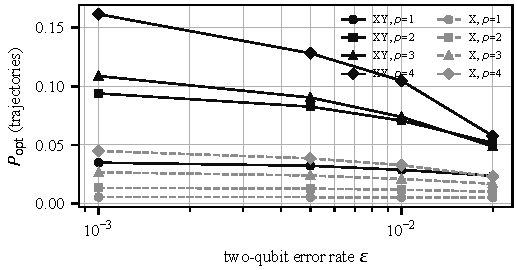
\includegraphics[width=\columnwidth]{fig_noise.pdf}
\caption{Gate-level trajectory estimate of $P_{\mathrm{opt}}$ against the two-qubit error rate for each depth (\TrajInst{} instances, \TrajRuns{} runs per circuit).}
\label{fig:noise}
\end{figure}

\begin{table}[t]
\caption{$P_{\mathrm{opt}}$ at depth 4 under two-qubit noise: gate-level trajectories vs.\ global model (\TrajInst{} instances)}
\label{tab:noise}
\centering
\footnotesize
\setlength{\tabcolsep}{4pt}
\begin{tabular}{lcccc}
\toprule
 & \multicolumn{2}{c}{X mixer} & \multicolumn{2}{c}{XY mixer}\\
$\epsilon$ & traj. & global & traj. & global\\
\midrule
0.001 & 0.045 & 0.044 & 0.162 & 0.161\\
0.005 & 0.038 & 0.036 & 0.128 & 0.121\\
0.01 & 0.033 & 0.028 & 0.105 & 0.086\\
0.02 & 0.023 & 0.016 & 0.058 & 0.043\\
\bottomrule
\multicolumn{5}{l}{\scriptsize traj. = mean over \TrajRuns{} Pauli-error trajectories; global = model (\ref{eq:noise}).}\\
\end{tabular}
\end{table}

\subsection{Classical Baselines and Scaling}
Exhaustive search over the 81 one-hot plans took \ExactMs~ms per instance and is exact. The greedy rule produced a feasible plan in \GreedyFeas\% of instances and the optimal one in \GreedyOpt\%. A single short simulated-annealing run (60 sweeps) on the same QUBO reached the optimum in only \SAOpt\% of instances and a feasible plan in \SAFeas\%, in \SAMs~ms. It is a weak baseline at this budget, and more restarts would close the gap at negligible cost. Training one QAOA configuration up to $p=4$ took several seconds of simulation. At this size, QAOA is not competitive on time, and the comparison is about solution quality per circuit, not speed.

Table~\ref{tab:scale} shows the scaling run. As $G$ grows, the number of one-hot plans grows as $3^G$ and $P_{\mathrm{opt}}$ for uniform sampling falls to \ScaleUnisix{} at \ScaleMaxQ{} qubits. The XY mixer at $p=2$ kept $P_{\mathrm{opt}}=\ScaleXYsix$ at that size, while one training run took \ScaleXYmsSix~s of simulation, compared with \ScaleExactSix~ms for exhaustive search. Statevector cost doubles with each qubit, so exact simulation of this kind stops being practical well before the problem becomes hard classically. Fig.~\ref{fig:scale} plots the same data on a log scale. The XY mixer stayed above uniform one-hot sampling at every size, from \ScaleXYtwo{} at 6 qubits to \ScaleXYsix{} at \ScaleMaxQ{}. The X mixer at $p=2$ fell below uniform one-hot sampling from 12 qubits on (\ScaleXsix{} at \ScaleMaxQ{} qubits), because most of its probability sat on bitstrings that are not plans at all: its feasibility probability at \ScaleMaxQ{} qubits was \ScaleXfeasSix, against \ScaleXYfeasSix{} for the XY mixer. One of the ten 18-qubit instances had no feasible plan and was excluded.

\begin{figure}[t]
\centering
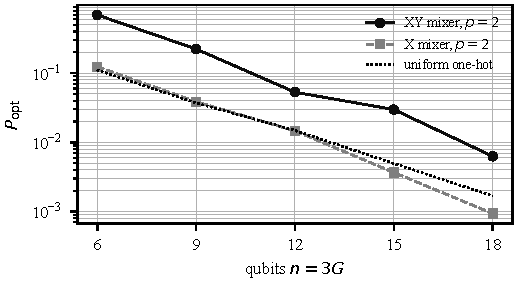
\includegraphics[width=\columnwidth]{fig_scale.pdf}
\caption{Probability of the optimal plan against problem size at depth 2 (log scale). The dotted line is uniform sampling of one-hot plans.}
\label{fig:scale}
\end{figure}

\begin{table}[t]
\caption{Scaling with the number of groups ($p=2$, mean objective)}
\label{tab:scale}
\centering
\footnotesize
\setlength{\tabcolsep}{2.4pt}
\begin{tabular}{ccccccccc}
\toprule
$G$ & $n$ & inst. & unif. & X $P_{\mathrm{opt}}$ & XY $P_{\mathrm{opt}}$ & XY $P_{\mathrm{feas}}$ & XY s & exact ms\\
\midrule
2 & 6 & 10 & 0.111 & 0.124 & 0.694 & 0.995 & 2.4 & 0.13\\
3 & 9 & 10 & 0.037 & 0.039 & 0.223 & 0.895 & 2.0 & 0.22\\
4 & 12 & 10 & 0.015 & 0.015 & 0.053 & 0.670 & 2.1 & 0.65\\
5 & 15 & 10 & 0.005 & 0.004 & 0.030 & 0.471 & 5.7 & 2.30\\
6 & 18 & 9 & 0.002 & 0.001 & 0.006 & 0.271 & 99.4 & 8.14\\
\bottomrule
\multicolumn{9}{l}{\scriptsize unif. = uniform one-hot $P_{\mathrm{opt}}$; XY s = simulated training time; inst. = feasible instances.}\\
\end{tabular}
\end{table}

\section{Discussion and Limitations}
Three points follow. First, building the constraint into the mixer helped more than any change to the training objective, although CVaR still improved the chance of finding the optimum within a fixed number of shots. For assignment problems with one-hot structure, the XY ansatz should be the default, and comparisons that use only the transverse-field mixer understate what QAOA can do. Second, the cost shift and penalty normalisation were necessary. Without them the energy is dominated by penalties and the optimiser learns feasibility but not cost. Third, classical methods solve these instances exactly in milliseconds. A realistic city-scale assignment with tens of groups and shelters would need hundreds of qubits and deep circuits, which is beyond the noise levels reported for current processors \cite{Harrigan2021,Bharti2022}.

The study has clear limits. The main results are noiseless, and the noise study in Section~\ref{sec:noise} ignores single-qubit and correlated errors, so the reported probabilities are upper bounds for hardware. The instances are small and come from one synthetic network, and accessibility constraints never bound because all three shelters are accessible. The pairwise capacity encoding is approximate in general. The XY mixer was Trotterised in a single fixed order, and we did not compile circuits to a hardware gate set or count depth after routing. Finally, the angle optimiser had a limited budget, so better angles may exist at higher depths.

For practitioners who want to try such formulations on hardware, our results suggest a short list of choices. Encode one-hot constraints in the mixer, not in penalties. Remove the per-group cost baseline and scale the Hamiltonian so that feasible energies span a unit interval, otherwise the angles must resolve differences that are tiny next to the penalties. Train on CVaR when the plan will be chosen as the best of a batch of shots. Finally, keep a classical exact or heuristic solver in the loop to verify every sample, because even the best variant here placed most of its probability on suboptimal plans for capacity-bound instances.

Several threats to validity remain. All variants were trained with the same optimiser budget and the same random starts, so the comparison between mixers is fair, but a larger budget could change the ranking at depth 4, where evaluations reached the cap of 750. The instances share one network and one disruption, so the binding and non-binding groups differ only in seeds, not in structure. The success@$N$ metric assumes independent shots from an exact distribution. On hardware, shot noise in the training objective and device noise would both lower it. Finally, the exhaustive reference makes the optimum known, which a real deployment would not have; the verification step we recommend only checks feasibility.

Future work will add single-qubit and correlated noise, transfer angles between instances, compare against slack-variable capacity encodings and test the XY ansatz on hardware through a cloud service.

\section{Conclusion}
On shelter-assignment instances drawn from a flood digital twin, a constraint-preserving ring-XY mixer gave QAOA a much higher probability of the optimal plan than the standard transverse-field mixer and kept most of the state on feasible plans at every depth. CVaR training narrowed the gap for the standard mixer but did not close it, and it made success within \Shots{} shots more reliable for both mixers. Exhaustive search solved the same instances exactly in about a millisecond, so the results show which formulation choices matter for future hardware experiments, not a present-day advantage.

\section*{Acknowledgment}
The authors thank the OpenStreetMap contributors and Open-Meteo for openly available data used by the digital twin.
In line with the IEEE policy on AI-generated content, the authors disclose that Claude (Anthropic) was used to help edit and restructure the text of all sections and to draft the simulation, experiment and plotting scripts. All experiments use the authors' own software and can be reproduced with fixed seeds. The authors checked every number, claim and reference and take full responsibility for the content.

\balance
\begin{thebibliography}{00}
\bibitem{Lucas2014} A. Lucas, ``Ising formulations of many NP problems,'' \textit{Front. Phys.}, vol. 2, Art. no. 5, 2014.
\bibitem{Glover2019} F. Glover, G. Kochenberger, and Y. Du, ``Quantum bridge analytics I: A tutorial on formulating and using QUBO models,'' \textit{4OR}, vol. 17, no. 4, pp. 335--371, 2019.
\bibitem{Cadelina2024} A. R. Cadeli\~{n}a \textit{et al.}, ``D-Wave implementation of quantum annealing for optimal resource allocation in disaster response operation of Marikina City,'' \textit{ECTI Trans. Comput. Inf. Technol.}, vol. 18, no. 1, pp. 24--33, 2024.
\bibitem{Abbas2024} A. Abbas \textit{et al.}, ``Challenges and opportunities in quantum optimization,'' \textit{Nat. Rev. Phys.}, vol. 6, pp. 718--735, 2024.
\bibitem{Farhi2014} E. Farhi, J. Goldstone, and S. Gutmann, ``A quantum approximate optimization algorithm,'' arXiv:1411.4028, 2014.
\bibitem{Hadfield2019} S. Hadfield, Z. Wang, B. O'Gorman, E. G. Rieffel, D. Venturelli, and R. Biswas, ``From the quantum approximate optimization algorithm to a quantum alternating operator ansatz,'' \textit{Algorithms}, vol. 12, no. 2, Art. no. 34, 2019.
\bibitem{WangZ2020} Z. Wang, N. C. Rubin, J. M. Dominy, and E. G. Rieffel, ``XY mixers: Analytical and numerical results for the quantum alternating operator ansatz,'' \textit{Phys. Rev. A}, vol. 101, no. 1, Art. no. 012320, 2020.
\bibitem{Fuchs2022} F. G. Fuchs, K. O. Lye, H. M. Nilsen, A. J. Stasik, and G. Sartor, ``Constraint preserving mixers for the quantum approximate optimization algorithm,'' \textit{Algorithms}, vol. 15, no. 6, Art. no. 202, 2022.
\bibitem{Barkoutsos2020} P. K. Barkoutsos, G. Nannicini, A. Robert, I. Tavernelli, and S. Woerner, ``Improving variational quantum optimization using CVaR,'' \textit{Quantum}, vol. 4, Art. no. 256, 2020.
\bibitem{Kirkpatrick1983} S. Kirkpatrick, C. D. Gelatt, and M. P. Vecchi, ``Optimization by simulated annealing,'' \textit{Science}, vol. 220, no. 4598, pp. 671--680, 1983.
\bibitem{Sherali1991} H. D. Sherali, T. B. Carter, and A. G. Hobeika, ``A location-allocation model and algorithm for evacuation planning under hurricane/flood conditions,'' \textit{Transp. Res. B, Methodol.}, vol. 25, no. 6, pp. 439--452, 1991.
\bibitem{Bartschi2019} A. B\"{a}rtschi and S. Eidenbenz, ``Deterministic preparation of Dicke states,'' in \textit{Fundamentals of Computation Theory} (LNCS, vol. 11651). Cham, Switzerland: Springer, 2019, pp. 126--139.
\bibitem{Zhou2020} L. Zhou, S.-T. Wang, S. Choi, H. Pichler, and M. D. Lukin, ``Quantum approximate optimization algorithm: Performance, mechanism, and implementation on near-term devices,'' \textit{Phys. Rev. X}, vol. 10, no. 2, Art. no. 021067, 2020.
\bibitem{Egger2021} D. J. Egger, J. Mare\v{c}ek, and S. Woerner, ``Warm-starting quantum optimization,'' \textit{Quantum}, vol. 5, Art. no. 479, 2021.
\bibitem{Harrigan2021} M. P. Harrigan \textit{et al.}, ``Quantum approximate optimization of non-planar graph problems on a planar superconducting processor,'' \textit{Nat. Phys.}, vol. 17, pp. 332--336, 2021.
\bibitem{Preskill2018} J. Preskill, ``Quantum computing in the NISQ era and beyond,'' \textit{Quantum}, vol. 2, Art. no. 79, 2018.
\bibitem{Bharti2022} K. Bharti \textit{et al.}, ``Noisy intermediate-scale quantum algorithms,'' \textit{Rev. Mod. Phys.}, vol. 94, no. 1, Art. no. 015004, 2022.
\bibitem{Powell1994} M. J. D. Powell, ``A direct search optimization method that models the objective and constraint functions by linear interpolation,'' in \textit{Advances in Optimization and Numerical Analysis}, S. Gomez and J.-P. Hennart, Eds. Dordrecht, The Netherlands: Kluwer, 1994, pp. 51--67.
\end{thebibliography}

\end{document}
